\section{Branch Prediction}

\frame{\tableofcontents[currentsection]}

\begin{frame}
  \frametitle{How Does The CPU Execute Instructions?}
  \begin{itemize}
    \item CPU receives stream of instructions
    \item CPU executes these instructions one after the other
          \begin{itemize}
            \item<2-> or, that's what it should look like
          \end{itemize}
  \end{itemize}
  \vskip5mm
  \begin{center}
    \begin{tikzpicture}[instruction/.style={font=\ttfamily\scshape,minimum height=.75cm,minimum width=1.5cm,draw,fill=blue!50,drop shadow}]
      \node[instruction] (instruction 1) {\dots};
      \node[instruction,anchor=north west] (instruction 2) at (instruction 1.north east) {mov};
      \node[instruction,anchor=north west] (instruction 3) at (instruction 2.north east) {add};
      \node[instruction,anchor=north west] (instruction 4) at (instruction 3.north east) {mul};
      \node[instruction,anchor=north west] (instruction 5) at (instruction 4.north east) {mov};
      \node[instruction,anchor=north west] (instruction 6) at (instruction 5.north east) {\dots};
    \end{tikzpicture}
  \end{center}
\end{frame}

\begin{frame}
  \frametitle{Car Assembly Analogy}
  \begin{itemize}
    \item Imagine car assembly line
    \item Assembling a car takes many phases
          \begin{itemize}
            \item E.g.~3 phases named A, B, C
          \end{itemize}
    \item Does it make sense to wait for one car to be finished before starting another?
    \item Assembly of 3 cars takes 9 time units
    \item Assembly of $n$ cars takes $3n$ steps
  \end{itemize}
  \begin{center}
    \begin{tikzpicture}[phase/.style={font=\scshape,minimum height=.75cm,minimum width=1cm},
                        phase a/.style={phase,fill=red!50},
                        phase b/.style={phase,fill=blue!50},
                        phase c/.style={phase,fill=green!50},]
      \node[phase a] (a1) {A};
      \node[phase b,anchor=north west] (b1) at (a1.north east) {B};
      \node[phase c,anchor=north west] (c1) at (b1.north east) {C};
      \node[phase a,anchor=north west] (a2) at (c1.north east) {A};
      \node[phase b,anchor=north west] (b2) at (a2.north east) {B};
      \node[phase c,anchor=north west] (c2) at (b2.north east) {C};
      \node[phase a,anchor=north west] (a3) at (c2.north east) {A};
      \node[phase b,anchor=north west] (b3) at (a3.north east) {B};
      \node[phase c,anchor=north west] (c3) at (b3.north east) {C};

      \foreach \i in {1,2,3} {
        \draw[|-|] ($ (a\i.south west) + (0,-0.1) $) -- ($ (c\i.south east) + (0,-0.1) $) node[midway,below,font=\small] {car \i};
      }

      \foreach[count=\i] \p in {a1,b1,c1,a2,b2,c2,a3,b3,c3} {
        \node[anchor=south,circle,draw,inner sep=1pt] at ($ (\p.north) + (0,0.1) $) {\tiny\i};
      }
    \end{tikzpicture}
  \end{center}
\end{frame}

\begin{frame}
  \frametitle{Car Assembly Analogy}
  \begin{itemize}
    \item Different phases of different cars can happen in parallel
    \item Start with car 2 as soon as car 1 finishes phase A
    \item Assembly of 3 cars takes 5 steps
    \item Assembly of $n$ cars takes $n+2$ steps
  \end{itemize}
  \begin{center}
    \begin{tikzpicture}[phase/.style={font=\scshape,minimum height=.75cm,minimum width=1cm},
                        phase a/.style={phase,fill=red!50},
                        phase b/.style={phase,fill=blue!50},
                        phase c/.style={phase,fill=green!50},]
      \node[phase a] (a1) {A};
      \node[phase b,anchor=north west] (b1) at (a1.north east) {B};
      \node[phase c,anchor=north west] (c1) at (b1.north east) {C};
      \node[phase a,anchor=north west] (a2) at (a1.south east) {A};
      \node[phase b,anchor=north west] (b2) at (b1.south east) {B};
      \node[phase c,anchor=north west] (c2) at (c1.south east) {C};
      \node[phase a,anchor=north west] (a3) at (a2.south east) {A};
      \node[phase b,anchor=north west] (b3) at (b2.south east) {B};
      \node[phase c,anchor=north west] (c3) at (c2.south east) {C};

      \foreach[count=\i] \pid in {a1,b1,c1,c2,c3} {
        \path let \p1=(a1.north), \p2=(\pid.north) in
              node[anchor=south,circle,draw,inner sep=1pt] at ($ (\x2,\y1) + (0,0.1) $) {\tiny\i};
      }
    \end{tikzpicture}
  \end{center}
\end{frame}

\begin{frame}
  \frametitle{Pipelining}
  \begin{itemize}
    \item Same approach is used by CPUs
    \item Instructions are split up in different stages (say 4)
    \item Different stages of different instructions execute in parallel
  \end{itemize}
  \vskip5mm
  \begin{overprint}
    \onslide<1>
    \begin{center}
      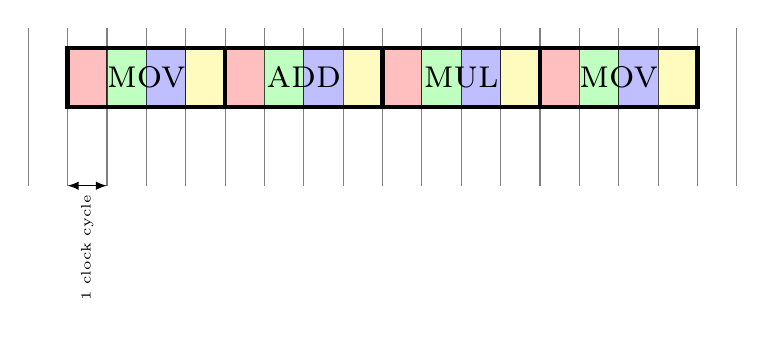
\begin{tikzpicture}[phase/.style={opacity=.5}]
        \foreach[evaluate={\i*0.5} as \x] \i in {-1,...,17} {
          \draw[gray,thin] (\x,-1) -- (\x,1);
        }

        \draw[latex-latex] (0,-1) -- (0.5,-1) node[rotate=90,left,midway,font=\tiny] {1 clock cycle};

        \foreach[count=\i,evaluate={(\i-1)*2} as \x] \instruction in {mov,add,mul,mov} {
          \begin{scope}[xshift=\x cm]
            \draw[phase,fill=red!50] (0,0) rectangle ++(0.5,0.75);
            \draw[phase,fill=green!50] (0.5,0) rectangle ++(0.5,0.75);
            \draw[phase,fill=blue!50] (1,0) rectangle ++(0.5,0.75);
            \draw[phase,fill=yellow!50] (1.5,0) rectangle ++(0.5,0.75);
            \draw[ultra thick] (0,0) rectangle ++(2,0.75);
            \node[font=\scshape] at (1,0.75/2) {\Large\instruction};
          \end{scope}
        }
      \end{tikzpicture}
    \end{center}

    \onslide<2>
    \begin{center}
      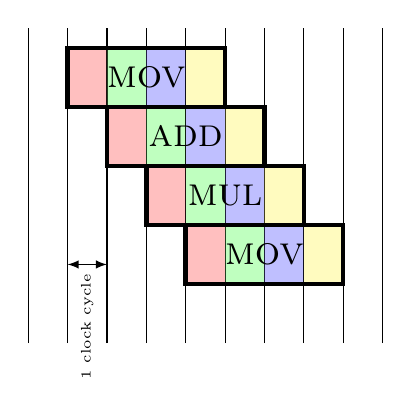
\begin{tikzpicture}[phase/.style={opacity=.5}]
        \foreach[evaluate={\i*0.5} as \x] \i in {-1,...,8} {
          \draw (\x,-3) -- (\x,1);
        }

        \draw[latex-latex] (0,-2) -- (0.5,-2) node[rotate=90,left,midway,font=\tiny] {1 clock cycle};

        \foreach[count=\i,evaluate={(\i-1)*0.5} as \x,evaluate={-(\i-1)*0.75} as \y] \instruction in {mov,add,mul,mov} {
          \begin{scope}[xshift=\x cm,yshift =\y cm]
            \draw[phase,fill=red!50] (0,0) rectangle ++(0.5,0.75);
            \draw[phase,fill=green!50] (0.5,0) rectangle ++(0.5,0.75);
            \draw[phase,fill=blue!50] (1,0) rectangle ++(0.5,0.75);
            \draw[phase,fill=yellow!50] (1.5,0) rectangle ++(0.5,0.75);
            \draw[ultra thick] (0,0) rectangle ++(2,0.75);
            \node[font=\scshape] at (1,0.75/2) {\Large\instruction};
          \end{scope}
        }
      \end{tikzpicture}
    \end{center}
  \end{overprint}
\end{frame}

\begin{frame}
  \frametitle{Pipelining}
  \begin{itemize}
    \item Allows instructions to overlap in time
    \item Instructions are executed in parallel
    \item To maximise efficiency, the pipeline needs to be fed new instructions at all times
  \end{itemize}
\end{frame}

\begin{frame}
  \frametitle{Conditionals}
  \code[language=c++14,width=.4\linewidth,font=\small]{conditional.cpp}
  \begin{itemize}
    \item Conditionals cause trouble
    \item \texttt{cond} determines which path to take
          \begin{itemize}
            \item We cannot add new instructions to pipeline as long as we don't know the value of \texttt{cond}
            \item Pipeline will be completely emptied before \texttt{a} or \texttt{b} executes
          \end{itemize}
    \item Really bad for performance
  \end{itemize}
\end{frame}

\begin{frame}
  \frametitle{Branch Prediction}
  \begin{itemize}
    \item Solution: try to guess which path will be taken
    \item CPU picks path and starts executing as if there was no \texttt{if}
    \item If chosen path turns out to be wrong path, CPU needs to undo everything
          \begin{itemize}
            \item Good performance if guess was good
            \item Bad performance if guess was bad
          \end{itemize}
    \item How does CPU maximise good guesses?
    \item Many different approaches possible
  \end{itemize}
\end{frame}

\begin{frame}
  \frametitle{Static Branch Prediction}
  \begin{itemize}
    \item CPU always guesses the then-branch will be taken
    \item Programmer needs to write program so that then-branch is more probable
  \end{itemize}
  \vskip5mm
  \begin{overprint}
    \onslide<1>
    \code[language=c++14,code=\small]{static-branch-prediction.cpp}

    \onslide<2>
    \code[language=c++14,code=\small]{static-branch-prediction2.cpp}
  \end{overprint}
\end{frame}

\begin{frame}
  \frametitle{Dynamic Branch Prediction}
  \begin{itemize}
    \item CPU keeps count at runtime
    \item Tries to detect patterns
  \end{itemize}
  \vskip5mm
  \begin{overprint}
    \onslide<1>
    \code[language=c++14,code=\small,width=.9\linewidth]{dynamic-branch-prediction.cpp}

    \onslide<2>
    \code[language=c++14,code=\small,width=.9\linewidth]{dynamic-branch-prediction2.cpp}
  \end{overprint}
\end{frame}

\begin{frame}
  \frametitle{Example Benchmark}
  \begin{center}
    \begin{tabular}{cc}
      \textbf{Pattern} & \textbf{Time} \\
      \toprule
      \texttt{F} & 5746 \\ % 0
      \texttt{FT} & 6264 \\ % 1
      \texttt{FFTT} & 5893 \\ % 2
      \texttt{FTTT} & 5808 \\ % 3
      \texttt{FFFTTTT} & 8692 \\ % 4
      \texttt{FTFTTTTT} & 7465 \\ % 5
      \texttt{FFTTTTTT} & 7832 \\ % 6
      \texttt{FTTTTTTTF} & 7059 \\ % 7
      \texttt{FFFFFFFFTTTTTTTT} & 8355 \\ % 8
      \texttt{FTFTFTFTTTTTTTTT} & 7814 \\ % 9
      \texttt{FFTTFFTTTTTTTTTT} & 7355 \\ % 10
      \texttt{FTTTFTTTTTTTTTTT} & 6931 \\ % 11
      \texttt{FFFFTTTTTTTTTTTT} & 7735 \\ % 12
    \end{tabular}
  \end{center}
  \begin{center} \bfseries
    Measurements done on Core i7 6700, 3.4GHz
  \end{center}
\end{frame}

%%% Local Variables:
%%% mode: latex
%%% TeX-master: "performance"
%%% End:
